%  LaTeX support: latex@mdpi.com 
%  For support, please attach all files needed for compiling as well as the log file, and specify your operating system, LaTeX version, and LaTeX editor.

%=================================================================

\documentclass[algorithms,article,accept,oneauthor]{Definitions/mdpi} 
\usepackage{microtype}
\usepackage{graphicx}
\usepackage{natbib}
\usepackage{xcolor}
\usepackage{amssymb,amsmath}
\usepackage{booktabs} % for professional tables
%\newtheorem{definition}{Definition}
% \newtheorem{theorem}{Theorem}
\DeclareMathOperator*{\argmin}{arg\, min} 
\DeclareMathOperator*{\argmax}{arg\, max} 
\newcommand{\revised}[1]{{\color{red}#1}}

% \usepackage{hyperref}
\usepackage[ruled,vlined,algo2e,linesnumbered]{algorithm2e}
\setlength{\algoheightrule}{1pt} % thickness of the rules above and below
\setlength{\algotitleheightrule}{0.5pt}

%\documentclass[preprints,article,submit,pdftex,moreauthors]{Definitions/mdpi} 
% For posting an early version of this manuscript as a preprint, you may use "preprints" as the journal. Changing "submit" to "accept" before posting will remove line numbers.

% Below journals will use APA reference format:
% admsci, aieduc, behavsci, businesses, econometrics, economies, education, ejihpe, famsci, games, humans, ijcs, ijfs, jintelligence, journalmedia, jrfm, jsam, languages, peacestud, psycholint, publications, tourismhosp, youth

% Below journals will use Chicago reference format:
% arts, genealogy, histories, humanities, laws, literature, religions, risks, socsci

%--------------------
% Class Options:
%--------------------
%----------
% journal
%----------
% Choose between the following MDPI journals:
% accountaudit, acoustics, actuators, addictions, adhesives, admsci, adolescents, aerobiology, aerospace, agriculture, agriengineering, agrochemicals, agronomy, ai, aichem, aieduc, aieng, aimater, aimed, aipa, air, aisens, algorithms, allergies, alloys, amh, analog, analytica, analytics, anatomia, anesthres, animals, antibiotics, antibodies, antioxidants, applbiosci, appliedchem, appliedmath, appliedphys, applmech, applmicrobiol, applnano, applsci, aquacj, architecture, arm, arthropoda, arts, asc, asi, astronautics, astronomy, atmosphere, atoms, audiolres, automation, axioms, bacteria, batteries, bdcc, behavsci, beverages, biochem, bioengineering, biologics, biology, biomass, biomechanics, biomed, biomedicines, biomedinformatics, biomimetics, biomolecules, biophysica, bioresourbioprod, biosensors, biosphere, biotech, birds, blockchains, bloods, blsf, brainsci, breath, buildings, businesses, cancers, carbon, cardio, cardiogenetics, cardiovascmed, catalysts, cells, ceramics, challenges, chemengineering, chemistry, chemosensors, chemproc, children, chips, cimb, civileng, cleantechnol, climate, clinbioenerg, clinpract, clockssleep, cmd, cmtr, coasts, coatings, colloids, colorants, commodities, complexities, complications, compounds, computation, computers, condensedmatter, conservation, constrmater, cosmetics, covid, crops, cryo, cryptography, crystals, csmf, ctn, culture, curroncol, cyber, dairy, data, ddc, dentistry, dermato, dermatopathology, designs, devices, dhi, diabetology, diagnostics, dietetics, digital, disabilities, diseases, diversity, dna, drones, dynamics, earth, ebj, ecm, ecologies, econometrics, economies, edm, education, eesp, ejihpe, electricity, electrochem, electronicmat, electronics, encyclopedia, endocrines, energies, eng, engproc, entomology, entropy, environments, environremediat, epidemiologia, epigenomes, esa, est, famsci, fermentation, fibers, fintech, fire, fishes, fluids, foods, forecasting, forensicsci, forests, fossstud, foundations, fractalfract, fuels, future, futureinternet, futurepharmacol, futurephys, futuretransp, galaxies, games, gases, gastroent, gastrointestdisord, gastronomy, gels, genealogy, genes, geographies, geohazards, geomatics, geometry, geosciences, geotechnics, geriatrics, germs, glacies, grasses, green, greenhealth, gucdd, hardware, hazardousmatters, healthcare, hearts, hemato, hematolrep, hep, heritage, higheredu, highthroughput, histories, horticulturae, hospitals, humanities, humans, hydrobiology, hydrogen, hydrology, hydropower, hygiene, idr, iic, ijcs, ijem, ijerph, ijfs, ijgi, ijmd, ijms, ijns, ijom, ijpb, ijt, ijtm, ijtpp, ime, immuno, informatics, information, infrastructures, inorganics, insects, instruments, inventions, iot, j, jaestheticmed, jal, jcdd, jcm, jcp, jcrm, jcs, jcto, jdad, jdb, jdream, jemr, jeta, jfb, jfmk, jgbg, jgg, jimaging, jintelligence, jlpea, jmahp, jmmp, jmms, jmp, jmse, jne, jnt, jof, joi, joitmc, joma, jop, joptm, jor, journalmedia, jox, jpbi, jphytomed, jpm, jrfm, jsam, jsan, jtaer, jvd, jzbg, kidneydial, kinasesphosphatases, knowledge, labmed, laboratories, lae, land, languages, laws, life, lights, limnolrev, lipidology, liquids, literature, livers, logics, logistics, lubricants, lymphatics, machines, macromol, magnetism, magnetochemistry, make, marinedrugs, materials, materproc, mathematics, mca, measurements, medicina, medicines, medsci, membranes, merits, metabolites, metals, meteorology, methane, metrics, metrology, micro, microarrays, microbiolres, microelectronics, micromachines, microorganisms, microplastics, microwave, minerals, mining, mmphys, modelling, molbank, molecules, mps, msf, mti, multimedia, muscles, nanoenergyadv, nanomanufacturing, nanomaterials, ncrna, ndt, network, neuroglia, neuroimaging, neurolint, neurosci, nitrogen, notspecified, nursrep, nutraceuticals, nutrients, obesities, occuphealth, oceans, ohbm, onco, optics, oral, organics, organoids, osteology, oxygen, pandemics, parasites, parasitologia, particles, pathogens, pathophysiology, peacestud, pediatrrep, pets, pharmaceuticals, pharmaceutics, pharmacoepidemiology, pharmacy, philosophies, photochem, photonics, phycology, physchem, physics, physiologia, plants, plasma, platforms, pollutants, polymers, polysaccharides, populations, poultry, powders, precipitation, precisoncol, preprints, proceedings, processes, prosthesis, proteomes, psf, psychiatryint, psychoactives, psycholint, publications, purification, quantumrep, quaternary, qubs, radiation, rdt, reactions, realestate, receptors, recycling, regeneration, religions, remotesensing, reports, reprodmed, resources, rheumato, risks, rjpm, robotics, rsee, ruminants, safety, sci, scipharm, sclerosis, seeds, sensors, separations, sexes, shi, signals, sinusitis, siuj, skins, smartcities, sna, societies, socsci, software, soilsystems, solar, solids, spectroscj, sports, standards, stats, std, stratsediment, stresses, surfaces, surgeries, suschem, sustainability, symmetry, synbio, systems, tae, targets, taxonomy, technologies, telecom, test, textiles, thalassrep, therapeutics, thermo, timespace, tomography, tourismhosp, toxics, toxins, tph, transplantology, transportation, traumacare, traumas, tri, tropicalmed, universe, urbansci, uro, vaccines, vehicles, venereology, vetsci, vibration, virtualworlds, viruses, vision, waste, water, welding, wem, wevj, wild, wind, women, world, youth, zoonoticdis

%---------
% article
%---------
% The default type of manuscript is "article", but can be replaced by: 
% abstract, addendum, article, benchmark, book, bookreview, briefcommunication, briefreport, casereport, changes, clinicopathologicalchallenge, comment, commentary, communication, conceptpaper, conferenceproceedings, correction, conferencereport, creative, datadescriptor, discussion, entry, expressionofconcern, extendedabstract, editorial, essay, erratum, fieldguide, hypothesis, interestingimages, letter, meetingreport, monograph, newbookreceived, obituary, opinion, proceedingpaper, projectreport, reply, retraction, review, perspective, protocol, shortnote, studyprotocol, supfile, systematicreview, technicalnote, viewpoint, guidelines, registeredreport, tutorial,  giantsinurology, urologyaroundtheworld
% supfile = supplementary materials

%----------
% submit
%----------
% The class option "submit" will be changed to "accept" by the Editorial Office when the paper is accepted. This will only make changes to the frontpage (e.g., the logo of the journal will get visible), the headings, and the copyright information. Also, line numbering will be removed. Journal info and pagination for accepted papers will also be assigned by the Editorial Office.

%------------------
% moreauthors
%------------------
% If there is only one author the class option oneauthor should be used. Otherwise use the class option moreauthors.

%---------
% pdftex
%---------
% The option pdftex is for use with pdfLaTeX. Remove "pdftex" for (1) compiling with LaTeX & dvi2pdf (if eps figures are used) or for (2) compiling with XeLaTeX.

%=================================================================
% MDPI internal commands - do not modify
\firstpage{1} 
\makeatletter 
\setcounter{page}{\@firstpage} 
\makeatother
\pubvolume{1}
\issuenum{1}
\articlenumber{0}
\pubyear{2026}
\copyrightyear{2026}
\externaleditor{Firstname Lastname} % More than 1 editor, please add `` and '' before the last editor name
\datereceived{15 June 2026} 
\daterevised{31 August 2026} % Comment out if no revised date
\dateaccepted{2 September 2026} 
\datepublished{ } 
%\datecorrected{} % For corrected papers: "Corrected: XXX" date in the original paper.
%\dateretracted{} % For retracted papers: "Retracted: XXX" date in the original paper.
%\doinum{} % Used for some special journals, like molbank
%\pdfoutput=1 % Uncommented for upload to arXiv.org
%\CorrStatement{yes}  % For updates
%\longauthorlist{yes} % For many authors that exceed the left citation part
%\IsAssociation{yes} % For association journals

%=================================================================
% Add packages and commands here. The following packages are loaded in our class file: fontenc, inputenc, calc, indentfirst, fancyhdr, graphicx, epstopdf, lastpage, ifthen, float, amsmath, amssymb, lineno, setspace, enumitem, mathpazo, booktabs, titlesec, etoolbox, tabto, xcolor, colortbl, soul, multirow, microtype, tikz, totcount, changepage, attrib, upgreek, array, tabularx, pbox, ragged2e, tocloft, marginnote, marginfix, enotez, amsthm, natbib, hyperref, cleveref, scrextend, url, geometry, newfloat, caption, draftwatermark, seqsplit
% cleveref: load \crefname definitions after \begin{document}

%=================================================================
% Please use the following mathematics environments: Theorem, Lemma, Corollary, Proposition, Characterization, Property, Problem, Example, ExamplesandDefinitions, Hypothesis, Remark, Definition, Notation, Assumption
%% For proofs, please use the proof environment (the amsthm package is loaded by the MDPI class).

%=================================================================
% Full title of the paper (Capitalized)
\Title{Finite Sample Complexity Analysis of Binary Segmentation}

% Author Orchid ID: enter ID or remove command
\newcommand{\orcidauthorA}{0000-0002-3146-0865} % Add \orcidA{} behind the author's name
%\newcommand{\orcidauthorB}{0000-0000-0000-000X} % Add \orcidB{} behind the author's name

% Authors, for the paper (add full first names)
\Author{\hl{Toby Dylan Hocking}
 \orcidA{}}

%\longauthorlist{yes}

% MDPI internal command: Authors, for metadata in PDF
\AuthorNames{Toby Hocking}

%\longauthorlist{yes}

% Affiliations / Addresses (Add [1] after \address if there is only one affiliation.)
\address[1]{\hl{Université de Sherbrooke, Département d'informatique, 2500 Boulevard de l'Université, Sherbrooke, QC, J1K-2R1, Canada;} 
 toby.dylan.hocking@usherbrooke.ca}


% Current address and/or shared authorship
%\firstnote{Current address: Affiliation.}  
% Current address should not be the same as any items in the Affiliation section.

%\secondnote{These authors contributed equally to this work.}
% The commands \thirdnote{} till \eighthnote{} are available for further notes.

%\simplesumm{} % Simple summary

%\conference{} % An extended version of a conference paper

% Abstract (Do not insert blank lines, i.e. \\) 
\abstract{Binary segmentation is the classic greedy algorithm which recursively splits a sequential data set by optimizing some loss or likelihood function.
Binary segmentation is widely used for changepoint detection in data sets measured over space or time, and as a sub-routine for decision tree learning.
In theory it should be extremely fast for $N$ data and $K$ splits, $O(N K)$ in the worst case, and $O(N \log K)$ in the best case. 
In this paper we 
describe new methods for analyzing the time and space complexity of binary segmentation for a given finite $N$, $K$, and minimum segment length parameter.
First, we describe algorithms that can be used to compute the best and worst case number of splits the algorithm must consider.
Second, we describe synthetic data that achieve the best and worst case and which can be used to test for correct implementation of the algorithm.
Finally, we provide an empirical analysis of real data which suggests that binary segmentation is often close to optimal speed in~practice.
}

% Keywords
\keyword{change-point detection; segmentation; heuristics} 

% The fields PACS, MSC, and JEL may be left empty or commented out if not applicable
%\PACS{J0101}
%\MSC{}
%\JEL{}

%%%%%%%%%%%%%%%%%%%%%%%%%%%%%%%%%%%%%%%%%%
% Only for the journal Diversity
%\LSID{\url{http://}}

%%%%%%%%%%%%%%%%%%%%%%%%%%%%%%%%%%%%%%%%%%
% Only for the journal Applied Sciences
%\featuredapplication{Authors are encouraged to provide a concise description of the specific application or a potential application of the work. This section is not mandatory.}
%%%%%%%%%%%%%%%%%%%%%%%%%%%%%%%%%%%%%%%%%%

%%%%%%%%%%%%%%%%%%%%%%%%%%%%%%%%%%%%%%%%%%
% Only for the journal Data
%\dataset{DOI number or link to the deposited data set if the data set is published separately. If the data set shall be published as a supplement to this paper, this field will be filled by the journal editors. In this case, please submit the data set as a supplement.}
%\datasetlicense{License under which the data set is made available (CC0, CC-BY, CC-BY-SA, CC-BY-NC, etc.)}

%%%%%%%%%%%%%%%%%%%%%%%%%%%%%%%%%%%%%%%%%%
% Only for the journal BioTech, Fishes, Neuroimaging and Toxins
%\keycontribution{The breakthroughs or highlights of the manuscript. Authors can write one or two sentences to describe the most important part of the paper.}

%%%%%%%%%%%%%%%%%%%%%%%%%%%%%%%%%%%%%%%%%%
% Only for the journal Encyclopedia
%\encyclopediadef{For entry manuscripts only: please provide a brief overview of the entry title instead of an abstract.}

%%%%%%%%%%%%%%%%%%%%%%%%%%%%%%%%%%%%%%%%%%
% Different journals have different requirements. Please check the specific journal guidelines in the "Instructions for Authors" on the journal's official website.
%\addhighlights{yes}
%\renewcommand{\addhighlights}{%
%
%\noindent The goal is to increase the discoverability and readability of the article via search engines and other scholars. Highlights should not be a copy of the abstract, but a simple text allowing the reader to quickly and simplified find out what the article is about and what can be cited from it. Each of these parts should be devoted up to 2~bullet points.\vspace{3pt}\\
%\textbf{What are the main findings?}
% \begin{itemize}[labelsep=2.5mm,topsep=-3pt]
% \item First bullet.
% \item Second bullet.
% \end{itemize}\vspace{3pt}
%\textbf{What are the implications of the main findings?}
% \begin{itemize}[labelsep=2.5mm,topsep=-3pt]
% \item First bullet.
% \item Second bullet.
% \end{itemize}
%}

%%%%%%%%%%%%%%%%%%%%%%%%%%%%%%%%%%%%%%%%%%
\begin{document}


\section{Introduction}
\label{sec:introduction}



Data sequences are measured over time or space in many fields of study such as genomics~\citep{olshen2004circular}, oceanography~\citep{killick2010detection}, finance~\citep{fryzlewicz2014wild}, and neuroscience~\citep{Jewell2019}. 
In the analysis of such data, an important step involves detection of abrupt changes in the data distribution over time or space.
In this context, dynamic programming algorithms can be used to compute a globally optimal set of changes and segment-specific parameters for some loss or likelihood (even though the optimization problem is non-convex). 
For computing a model with $K$ splits for $N$ data, classic dynamic programming algorithms include the $O(K N^2)$ time algorithm of~\citet{segment-neighborhood} and the $O(N^2)$ algorithm of~\citet{Jackson2005}.
Since these classic algorithms are too slow for large $N$, new algorithms using pruning rules have been proposed to decrease computation time to $O(N\log N)$, while maintaining optimality~\citep{Maidstone2016}. 
However even these new optimal algorithms are not fast enough for some applications, so an alternative is the classic binary segmentation heuristic~\citep{binary-segmentation}.
Binary segmentation is not guaranteed to compute an optimal set of changepoints, but it can be extremely fast.
An entire regularization path of models from 0 to $K$ splits can be computed in worst case $O(N K)$, best case $O(N\log K)$ time.
Our paper provides a new method for analyzing the amount of computation that binary segmentation must do for a finite $N$ and $K$ (in the best and worst cases, as well as in real data sets).



\subsection{Related Work}
\label{sec:related-work}

The classic binary segmentation heuristic algorithm is originally attributed to~\citet{binary-segmentation}.
It involves recursively searching a sequential data set for the best split point, given previously chosen split points (Figure~\ref{fig:synthetic}).
More recent variants of binary segmentation have been proposed, such as searching random intervals~\citep{fryzlewicz2014wild, baranowski2019narrowest}.
Another idea is to limit the search to one changepoint each in a number of pre-defined seed intervals~\citep{kovacs2020seeded}.
Because a known limitation is detection of short segments in longer ones~\citep{venkatraman1992consistency}, more computationally intensive variants of binary segmentation have been proposed which involve searching for two split points simultaneously~\citep{levin1985cusum,olshen2004circular}.
Binary segmentation is also an important sub-routine in decision tree learning algorithms such as CART~\citep{breiman1984classification} and Maximum Margin Interval Trees~\citep{Drouin2017}.
In each of the above algorithms there is a model complexity parameter (number of splits/segments), which needs to be appropriately chosen given the data.
This model selection problem can be solved using several unsupervised~\citep{Yao88, mBIC} as well as supervised methods which can be used in situations where labeled training data are available~\citep{Hocking2013icml, truong2017penalty}.


\begin{figure}[H]
    %\centering
    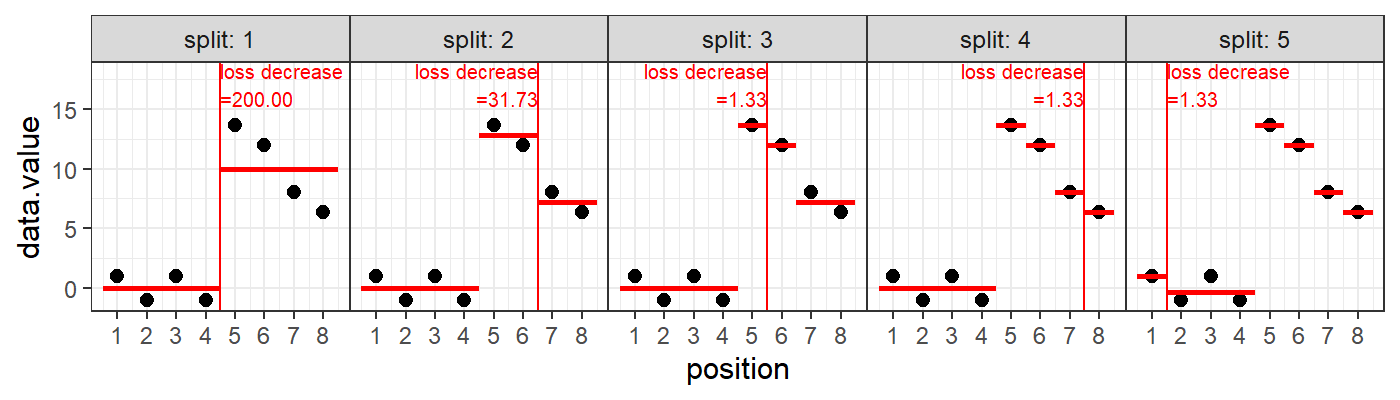
\includegraphics[width=\textwidth]{figure-synthetic.png}
    \vspace{-0.7cm}
    \caption{\hl{Demonstration} 
      of a binary segmentation algorithm on a simple synthetic data set (details in Section~\ref{ties-in-different-segments}) for which a tie-breaking rule is required to achieve the best case number of splits to consider.
      Black dots show data and red lines show the binary segmentation models.
    After the first two splits, the next three splits all have an equal loss decrease value (1.33), so the best case time complexity can be achieved with a tie-breaking rule that chooses a split which results in the smallest number of candidate splits to consider afterwards.}
    \label{fig:synthetic}
\end{figure}

The dynamic programming algorithm we propose to compute the best case number of splits for binary segmentation is similar to the idea of the optimal binary search tree, for which there are many classic algorithms~\citep{NAGARAJ19971}. 
For example~\citet{Knuth1971} described $O(n^3)$ and $O(n^2)$ optimal algorithms for a tree with $n$ nodes, as well as $O(n\log n)$ heuristic/approximate algorithms which are very fast but not guaranteed to compute the optimal tree.
Later~\citet{mehlhorn1975nearly} proved that the important heuristic was bisection, which always produces nearly optimal trees. %\url{https://en.wikipedia.org/wiki/Optimal_binary_search_tree}


\subsection{Contributions and Organization}
Our main contributions are new algorithms for finite sample time and space complexity analysis of binary segmentation.
We propose algorithms for computing the best and worst case number of splits that must be considered, which is proportional to overall computation time.
In Section~\ref{sec:bs-algo} we describe the classic binary segmentation algorithm, and provide new synthetic data examples that can be used for testing that the algorithm is correctly implemented.
In Section~\ref{sec:complexity-analysis} we propose new algorithms which can be used to compute the best and worst case number of splits for finite sample complexity analysis.
To the best of our knowledge this is the first time such finite sample complexity analysis has been described for binary segmentation with a minimum segment length parameter.
In Section~\ref{sec:results} we provide an empirical study of binary segmentation in several synthetic and real data sets.
Section~\ref{sec:discussion} concludes with a discussion of the significance and novelty of our~findings.

\section{Binary Segmentation Algorithm}
\label{sec:bs-algo}

In this section we provide an overview of how the binary segmentation algorithm works. 
We assume there is a sequence of $N$ data for which we want to compute $K$ splits/iterations (max number of segments is $K+1$). 
We further assume that each iteration splits a segment into two segments, each of minimum size $m$ (this is the minimum segment length parameter).
Finally, we assume there is a loss function $\ell$ that binary segmentation seeks to minimize (for example, common choices are the square loss or L1 loss for real-valued data, and the Poisson loss for non-negative integer count data).
The binary segmentation algorithm performs the following computations: 
(a) for any new segments, find the split which results in the best loss decrease; (b) store that segment/split in a container for future lookup; 
(c) look in that container for the  segment with best loss decrease and split it into two new segments; 
(d) repeat until the max number of splits $K$ is reached.

To analyze the time complexity of step (a) we use the number of candidate splits that must be considered to find the best loss decrease (Table~\ref{tab:best-worst-time}).
{Throughout the paper we use various synonyms for ``number of candidate splits that must be considered'': ``number of splits the algorithm must consider,''
``number of candidate split points,''
``number of candidate split evaluations,'' etc.
}
Note that this is a valid choice for finite sample time complexity analysis since the loss of each candidate split can be computed in amortized constant time for common loss functions including square/Poisson (and log-time for L1 loss).
The positions after which a change may occur in $N$ data are $\{m,\dots,N-m\}$ and the size of this set (number of candidate splits that must be considered) is
\begin{equation}
    \label{eq:g}
    g(N) = (N-2m+1)_+,
\end{equation}
where $(\cdot)_+$ is the positive part function (identity if argument is positive, otherwise zero).
For example, with min segment length $m=2$, we have $g(4)=1$ because, starting with four data, there is only one possible split (in the middle) that results in segments with at least two data.
We have $g(3)=g(2)=0$ with $m=2$ because segments of size 3 and 2 can not be split to yield two segments of at least size 2, so there are no candidate splits to consider.


\begin{table}[H]
    \caption{\hl{Counts} %MDPI: 1. We removed the vertical lines, and add top and bottom lines. Please confirm. 2. we add bold format as table header, please confirm.
 of best and worst case number of candidates to compute for $N=64$ data and min segment length $m=1$.
    Each row shows the number of candidates for a given split $K$ and tree depth $j$, along with the cumulative total.}
    \label{tab:best-worst-time}\setlength{\tabcolsep}{3mm} 
    %\centering
   % {\small
\begin{tabularx}{\textwidth}{cccccc}
\toprule
&& \multicolumn{2}{c}{\textbf{Best Case: Equal Splits}} &
\multicolumn{2}{c}{\textbf{Worst Case: Unequal Splits}} \\
\midrule
\textbf{\textit{j}} & \textbf{\textit{K}} & \textbf{This Iteration} & \textbf{Total} & \textbf{This Iteration} & \textbf{Total} \\
\midrule
1 & 0 & $N-1=63$  & $N-1=63$    & $N-1=63$ & $N-1=63$ \\
2 & 1 & $N-2=62$  & $2N-3=125$  & $N-2=62$ & $2N-3=125$ \\
  & 2 & $N/2-2=30$&             & $N-3=61$ & $3N-6=186$ \\
3 & 3 & $N/2-2=30$& $3N-7=185$  & $N-4=60$ & $4N-10=246$ \\
$\vdots$ &     $\vdots$ &     $\vdots$  & $\vdots$ & $\vdots$ & $\vdots$\\
4 & 7 & $N/4-2=14$& $4N-15=241$ & $N-8=56$ & $8N-36=476$ \\
$\vdots$ &     $\vdots$ &     $\vdots$  & $\vdots$ & $\vdots$ & $\vdots$ \\
7 & 63 & $N/32-2=0$&$7N-127=321$ & $N-64=0$ & $64N-2080=2016$ \\\bottomrule
\end{tabularx}
%}
\end{table}

To analyze the time and space complexity of steps (b) and (c) we need to specify what type of container is used. 
For efficiency the container should be a red-black tree or similar data structure which allows for constant time lookup of the item with best loss decrease, and insertion of a new item which is logarithmic in the container size.
For finite sample complexity analysis of steps (b) and (c) we therefore need to examine the container size before each insert (Table~\ref{tab:best-worst-storage}).
Note that in both steps (a) and (b) the ``best'' loss decrease must be identified.
In order for the algorithm to achieve the best case number of candidate splits considered, it must correctly perform tie-breaking, as explained in the next section.


\begin{table}[H]
    \caption{\hl{Table} %MDPI: 1. We removed the vertical lines, and add top and bottom lines. Please confirm. 2. we add bold format as table header, please confirm..
 of best and worst case storage, for $N=64$ data with min segment length $m=1$ and max number of segments/splits.
    Sizes before inserts columns show the size of the container before each insert operation (to analyze time complexity of the insert operation); size after iteration columns show the size of the container after each iteration (to analyze space complexity).
    Equal splits results in largest container size before inserts of $O(N)$, and worst case space complexity of $O(N)$. 
    Unequal splits result in the smallest container size before inserts (always zero), and best case storage (container size 1 after each iteration).}
    \label{tab:best-worst-storage}\setlength{\tabcolsep}{5mm} 
    %\centering
    %{\small
\begin{tabular}{ccccc}\toprule
     & \multicolumn{2}{c}{\textbf{Equal Splits}}    & \multicolumn{2}{c}{\textbf{Unequal Splits}}  \\
     \midrule
     &  \textbf{Sizes Before}  &   \textbf{Size After}   & \textbf{Sizes Before} & \textbf{Size After} \\
 \textbf{Iteration \textit{I}} &  \textbf{Inserts} &  \textbf{Iteration} &  \textbf{Inserts} &  \textbf{Iteration} \\
\midrule
 1 & 0   & 1 & 0 & 1 \\
 2 & \hl{0, 1} %MDPI: we add space after comma, please confirm all format in the whole text.
 & 2 & 0 & 1 \\ 
 3 & {1, 2} & 3 & 0 & 1 \\
$\vdots$ &     $\vdots$ &     $\vdots$  & $\vdots$ & $\vdots$ \\
32 & 30, 31 & 32 & 0 & 1 \\
33 &  none     & 31 & 0 & 1 \\
34 &  none     & 30 & 0 & 1 \\
$\vdots$ &     $\vdots$ &     $\vdots$  & $\vdots$ & $\vdots$ \\
62 &  none     & 2 & 0 & 1 \\
63 &  none     & 1 & 0 & 1\\\bottomrule
\end{tabular}
\end{table}


\subsection{Tie-Breaking Rules and Test Cases}
\label{ties-in-different-segments}
In this section we provide examples of simple synthetic data which have splits of equal loss, and thus require a tie-breaking rule in order to achieve the best case number of splits.
We begin by discussing the case of ties in split points within a segment, then we discuss the more complex case of ties in different segments that could be split.

\subsubsection{\highlighting{Ties in Split Points on a Segment}} %MDPI: we change it into headings-3, and add section number, please confirm. the same to following highlight section title.
 
When the binary segmentation algorithm considers a new segment to split, it must optimize over all possible split points, by taking the split that results in minimum loss. 
If there are several splits which each have the same minimum loss value, then to minimize the number of candidates to optimize over in the next step, the binary segmentation algorithm should first break ties using the number of split candidates which would need to be computed, then the distance from the start/end of the segment. 
A simple example is the data sequence [1, 2, \ldots, 8] with the L1 loss and min segment length $m=1$.
The optimal L1 loss values for the seven possible splits are [12, 10, 8, 8, 8, 10, 12], so there are three splits which result in the same min loss.
Each of these three splits has the same number of split candidates which would need to be computed during the next iteration, $g(3)+g(5)=g(4)+g(4)=6$.
The best case number of splits for future iterations is achieved if the algorithm chooses the split in the middle (two child segments of size 4).
{As discussed later, choosing the split in the middle is a heuristic, which is not guaranteed to achieve the best case number of candidate splits, but is sufficient to get within a constant factor.} More generally, let $\underline p$ be the segment start, $\overline p$ be the segment end, and $c\in\{\underline p, \dots, \overline p-1\}$ be a candidate split point.
The distance from split $c$ to the nearest start or end is
\begin{equation}
    D_c = \min\{ c-\underline p, \overline p-c-1 \}.
\end{equation}
\hl{Let} %MDPI: Please confirm whether this paragraph should be indented. please recheck all noindent under equations in following text.
 $\mathcal C$ be the set of splits to tie-break, with min loss and min number of split candidates which would need to be computed during the next iteration.
The best case tie-breaking rule chooses the split with maximal value for the distance to nearest start or end,
\vspace{12pt}
\begin{equation}
    c^* = \argmax_{c\in\mathcal C} D_c.
\end{equation}
In the example above, the segment start $\underline p=1$, end $\overline p=8$, and set of splits to tie-break $\mathcal C=\{3,4,5\}$. 
Distances are $D_3=2$, $D_4=3$, $D_5=2$, so the best split is therefore $c^* = 4$, which results in two segments of size 4.
This requires computing six new candidates in the next step (three on each of the two segments with four data), then four in the following steps (one on each of the four segments with two data), for a total of 10 candidates.
This is preferable to the other options, which result in a larger number of candidates (4 and 2 with segments of size 3 and 5; then 1, 2, 2 for segments of size 2, 2, 3; then 1 for final segment of size 2; total number of candidates 12).

\subsubsection{\highlighting{Ties in Different Segments That Could Be Split}} 
A flexible and efficient implementation of binary segmentation requires a container to store the different segments that could be split during each iteration. 
The segments in this container should be sorted by loss decrease values; the next segment to split should result in the largest loss decrease.
Similar to the discussion above about ties in split points on a segment, it is possible for there to be several segments which have the same loss decrease value. 
In this case, to achieve the best case number of splits to optimize over in subsequent iterations, the algorithm should again break ties in the same way. 
A simple synthetic data set for which this tie-breaking rule is necessary using the L2 square loss can be constructed in the following manner. 
% > matrix(data.vec,4)
%           [,1] [,2]      [,3] [,4]
% [1,]  2.598076    8 -2.598076   -8
% [2,] -2.598076    9  2.598076   -9
% [3,]  2.598076   11 -2.598076  -11
% [4,] -2.598076   12  2.598076  -12
First, let $a,b,x,\epsilon\in\mathbb R$ be real number parameters which will determine our synthetic data  $[a,-a,a,-a|b+\epsilon+x,b+\epsilon|b-\epsilon,b-\epsilon-x]$.
The idea is to choose a $b$ and $\epsilon$ large enough so that the first two splits happen at the vertical bar positions, resulting in three segments.
Then $a$ and $x$ can be chosen such that all three segments have an equal value for the best loss decrease. 
We chose $a=1$, $b=10$, $x=\sqrt{8/3}$, $\epsilon=2$, which results in the data shown in Figure~\ref{fig:synthetic}.
The algorithm proceeds as follows:
\begin{enumerate}[leftmargin=36pt,labelsep=16pt]
\item[Split~1:]
}] 7 candidates are considered; the best has a change after position 4. 
\item[Split~2:] Each of the two new children segments created from split 1 require computing the loss of 3 split candidates, for a total of 6 candidates considered.
Splitting the optimal segment results in a change after position 6, whereas the other segment with a loss decrease of 4/3 stays in the container. 
\item[Split~3:] Each of the two new children segments created from split 2 require computing the loss of 1 split candidate, for a total of 2 candidates considered.
Both new segments have a loss decrease of 4/3, so the container now has three segments with the same loss decrease value.
Tie-breaking is performed by minimizing the number of split candidates which would be required to be computed in the next iteration; the result is a change after position 5.
Two segments with the same loss decrease value remain in the container.
\item[Split~4:] Both of the two new children segments created from split 3 are of size 1, so cannot be split, and do not require any new split candidates to be computed.
The next split results in a change after position 7, and one segment remains in the container.
\item[Split~5:] Again no new split candidates are computed, and instead the last segment in the container is split, resulting in a change after position 1, and an empty container.
\end{enumerate}

\hl{Looking} %MDPI: we add indent, please confirm.
 at the example above, we see that the total number of split candidates considered is 15, which is indeed the best case for $N=8$ data, $K=5$ splits, and a min segment length of $m=1$.
In contrast if we had not implemented tie-breaking, and had instead chosen split 3 after position 1, then we would have computed two additional split candidates, for a total of 17.
The worst case would be achieved for the data sequence  \mbox{[$-$1, 1, $-$1, 1, $-$1, 1, $-$1, 1] which for $K=5$} splits would require computing the loss for a total of 25 split candidates. 
In the next section we describe methods that can be used to compute the best/worst case number of iterations for any data size $N$, number of splits $K$, and min segment length $m$.

\section{Finite Sample Complexity Analysis}
\label{sec:complexity-analysis}




We begin this section with an analysis of the number of candidate splits that must be considered when computing the maximum number of splits, $K=N-1$. 
For simplicity we first assume a min segment length of $m=1$ and that $N$ is a multiple of 2; we can let $N=2^J$ for some $J\in\{1,2,\dots\}$, for example $J=6
  \Rightarrow N=64$.
Then for any $j\in\{1,\dots,J+1\}$ if we do $K=2^{j-1}-1$ splits then the number of candidates that must be considered is shown in Table~\ref{tab:best-worst-time}.
In the best case, each split results in segments of equal size, and we have $Nj -2^j + 1 = N(1+\log_2 K) -2K +1\leq 1+N+N\log_2 K \Rightarrow O(N \log K)$ total candidates to consider.
In the worst case, each split results in segments of unequal sizes, and we have $NK - K(1+K)/2\leq NK \Rightarrow O(NK)$ total candidates to consider.
 
To store the previously computed best loss/split for each segment, we use a container with insert operations which are logarithmic in container size---if the container has $p$ items then an insert takes $O(\log p)$ time. 
In Table~\ref{tab:best-worst-storage} we therefore analyze the container size in the two extreme cases (equal and unequal splits). 
The ``sizes before inserts'' columns show $p$ before each insert (to analyze time complexity), and the ``size after iteration'' columns show $p$ after inserts (to analyze space complexity). 
For unequal splits, the total time is linear, and the total space is constant, because the container always stays at size 1.
For equal splits, the total time over all inserts is $-\log(K-1) + \sum_{p=1}^{K-1} 2\log p\in O(K\log K)$, which is smaller than the $O(N\log K)$ time for the split computation, so the container insert step is not a limiting factor for time complexity.
However for equal splits, the space complexity achieves the worst case, a max container size of $N/2$ segments for which we have already computed the best split point, but we have not yet split, at iteration $N/2$.
{The asymptotic size of the container is $O(N)$ (same as the input data), and there is no larger storage to consider, so the space complexity is reasonable even for very large data sizes $N$.
}

\subsection{New Dynamic Programming Algorithm for Computing Best Case Number of Candidate Splits}
\label{sec:time-complexity}

In the previous section we provided an overview of how the finite sample complexity analysis works for the special case of the data size being a multiple of 2.
{The worst case analysis (counting number of candidates for unequal splits) also works for the general case.
In particular, for min segment length $m$, the worst case is obtained when $m$ data are split off by themselves in each iteration.
The worst case number of candidates is therefore $\sum_{i=0}^{K-1} g(N-im)$.
However, the best case analysis does not work in the general case (equal splits do not always result in the best case for small $K$).}
In this section we describe a new algorithm which can be used to compute the best case  number of splits that must be considered for any data size $N$, number of splits $K$, and min segment length $m$.

Recall from (\ref{eq:g}) that $g(N)$ is the number of candidate splits which must be considered in order to find the optimal split on the segment of size $N$.
{Let $f(N,T)$ be the best number of candidates  computed after the segment of size $N\geq 1$ is split $T\geq 0$ times; the resulting segments are stored in the container, and the best feasible segment is then split, resulting in a model with at most $K=T+1$ splits (there may be fewer if min segment length $m>1$ and some segments are not feasible to split).
For $T$ times, $2T+1$ is the number of segments which are created and then searched for the best split point.


The geometric interpretation of $f(N,T)$ involves a binary tree with $T$ splits and $2T+1$ nodes, in which each node represents a segment with a certain size, and the size of each parent always equals the sum of sizes over the two children (Figure~\ref{fig:optimal-trees-some}). 
Computing $f(N,T)$ involves searching the space of all trees with root size $N$, $T$ splits, and $2T+1$ nodes, in order to find the tree with min cost, as quantified by summing $g(s)$ over all node sizes $s$ in the tree.
}

\begin{figure}[H]
    %\centering
  \hspace{-12pt}  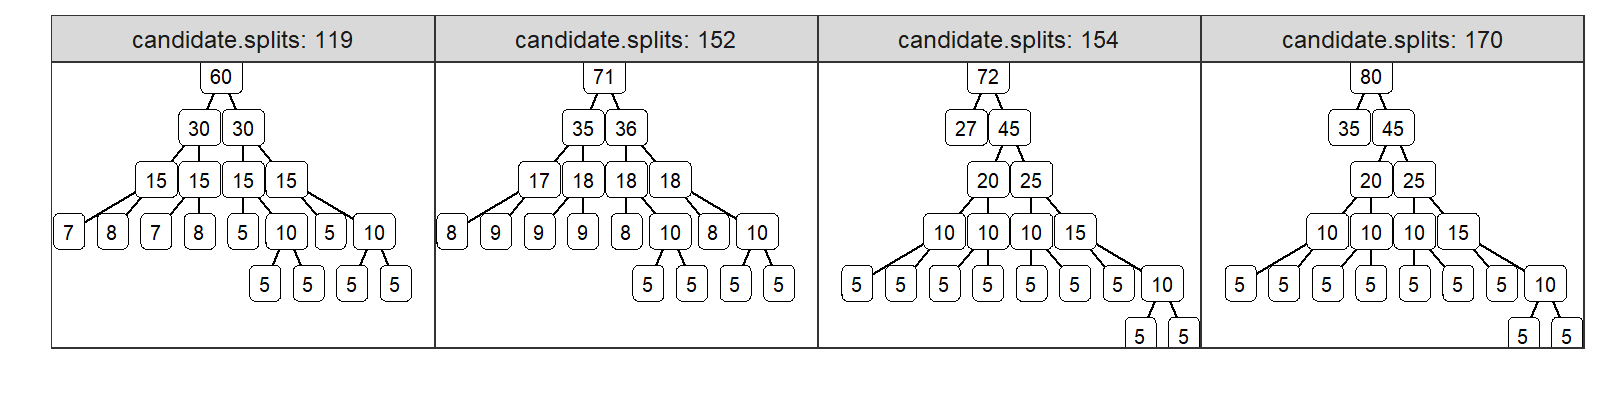
\includegraphics[width=\textwidth]{figure-optimal-trees-some.png}
 \vspace{-6pt}
    \caption{{Optimal}  binary trees constructed to determine optimal number of candidate splits for $N\in\{60,71,72,80\}$ data, which are split $T=9$ times, with min segment length $m=5$.
    Smaller $N$ values result in a balanced first split, whereas larger $N$ values result in an unbalanced first split (one small child with no splits, one large child with all remaining splits).}
    \label{fig:optimal-trees-some}
\end{figure}


For example, for $T=0$, there is only one segment (the original with all data) which is searched, with $f(N,0)=g(N)$ candidates considered, resulting in a model with $K=1$ split (2 segments).
This corresponds to a binary tree with one node and no splits.

For $T=1$, there are three segments searched (the original plus the two created after the first split), resulting in a model with $K=2$ splits (3 segments); the number of candidates to compute is
\begin{equation}
f(N,1) = g(N) + \min_{s\in\{m,\dots,N-m\}} f(s,0)+f(N-s, 0).
\end{equation}
The min above is over the split point $s$.
It can be efficiently computed in linear $O(N)$ time since each $f(N,0)=g(N)$ can be evaluated in constant time.
This corresponds to a binary tree with three nodes and one split.

For $T=2$, there are five segments searched (the original plus the four created after the first two splits), resulting in a model with $K=3$ splits (4 segments); the number of candidates to compute is
\begin{equation}
f(N,2) = g(N) + 
\min_{s\in\{m,\dots,N-2m\}} f(s,0)+f(N-s, 1)
\end{equation}
The split values $s$ have an upper bound of $N-2m$ to respect the min segment length $m$.
Assuming the each of the $f(N,1)$ values have been pre-computed, the min above can be efficiently computed in linear $O(N)$ time.
This corresponds to a binary tree with five nodes and two splits.

For $T=3$, there are seven segments searched (the original plus the six created after the first three splits), resulting in a model with $K=4$ splits (5 segments); the number of candidates to compute is
\begin{equation}
f(N,3) = g(N) + \min
\begin{cases}
\min_{s\in\{2m,\dots,N-2m\}} f(s,1)+f(N-s, 1)\\
\min_{s\in\{m,\dots,N-3m\}} f(s,0)+f(N-s, 2).
\end{cases}
\end{equation}
This corresponds to a binary tree with seven nodes and three splits.
Above, the first min is over tree topologies.
The first line in the min corresponds to splitting the left and right nodes once each, whereas the second line in the min corresponds to not splitting the left node, but splitting the right node twice.

% For a newly created segment with size $s$, there are $g(s)$ corresponding split candidates considered.
% To determine the optimal number of split candidates considered, we must


The key idea of our proposed algorithm is that $f(N,T)$ can be recursively computed.
For some ideal smaller number of changes $d\in\{0,\dots,T-1\}$, and for some ideal split size $s$, we have  $f(N,T) = g(N) + f(s,d) + f(N-s,T-d-1)$.
To compute this we need to search over all possible numbers of changes $d$ and split sizes $s$.
For any number of changes $d$, we have the following lower bound on the size $s$ due to the min segment length $m$,
\begin{equation}
\label{eq:s_lower_bound}
    s \geq (d+1)m.
\end{equation}

For the same reason we have the following upper bound,
\begin{equation}
    s \leq N+(d-T)m.
\end{equation}


For example consider computing $f(15,2)$ with min segment length of $m=3$. 
In that case we need to search over $f(s,0)+f(15-s,1)$ for seven sizes $s\in\{3,4,5,6,7,8,9\}$.
Additionally when the number of changes in the two child segments is the same, the symmetry of the problem implies the following stronger upper bound,
\begin{equation}
    d = (T-1)/2 \Rightarrow s\leq \lfloor N/2 \rfloor.
\end{equation}
For example consider computing $f(15,3)$ with min segment length of $m=3$.
In that case we need to search over $f(s,0)+f(15-s,2)$ for four sizes $s\in\{3,4,5,6\}$, and $f(s,1)+f(15-s,1)$ for just two sizes $s\in\{6,7\}$.
When there are $d$ changes the overall upper bound on $s$ is therefore
\begin{equation}
\label{eq:sbar}
    \overline s(N,T,d,m) = \begin{cases}
    N+(d-T)m & \text{ if } d < (T-1)/2,\\
    \lfloor N/2 \rfloor & \text{ if } d = (T-1)/2.
    \end{cases}
\end{equation}
For $N$ data, split $T$ times, with min segment length $m$, and any smaller number of changes $d<T$, we therefore have the following set of sizes $s$ to optimize over,
\begin{equation}
\label{eq:S}
    \mathcal S(N,T,d,m) = \{(d+1)m, \dots, \overline s(N,T,d,m)\}.
\end{equation}
The results above are combined into the theorem below, which gives an efficient and optimal method for computing the best case number of splits that need to be computed during binary segmentation.
\begin{Theorem}
Assume binary segmentation with $T$ splits, starting with a segment of $N$ data, with min segment length $m$.
The best case number of candidate splits that must be computed can be determined as follows.
First, for all $N$ we initialize $f(N,0) = g(N)$. 
Then, for all $T>0$ and for all $N$ we use the following dynamic programming update rule.
\begin{equation}
    \label{eq:f}
    f(N,T) = g(N) + 
    \min_{
    d\in\{0,\dots,\lfloor (T-1)/2\rfloor\}
    }
    \min_{
    s\in\mathcal S(N,T,d,m)
    }
    f(s,d) + f(N-s,T-d-1).
\end{equation}
\end{Theorem}
\begin{proof}
{First, $T$ takes values between 0 and $N-2$, which corresponds to models from 1 to $N-1$ splits (the max value is smaller if the min segment length $m>1$).
In (\ref{eq:S}), the lower bound $(d+1)m$ comes from (\ref{eq:s_lower_bound}): there must be $m$ data on a segment, so at least $2m$ data on a segment which must be split once, etc.
The upper bound~(\ref{eq:sbar}) comes from symmetry, meaning there is no need to check both $f(4,0)+f(6,0)$ and $f(6,0)+f(4,0)$, because they are of equal cost, etc.
Similarly the upper bound on $d$ in (\ref{eq:f}) comes from symmetry, meaning there is no need no check both $f(5,2)+f(5,0)$ and $f(5,0)+f(5,2)$, because they are of equal cost, etc.
Finally, the update rule avoids under-counting and double-counting candidates, by including a $g(s)$ term for each node in the corresponding binary tree.}
\end{proof}



\subsubsection*{\highlighting{Pseudo-Code and Complexity Analysis of Proposed Algorithm}} 
 
The dynamic programming algorithm is summarized in Algorithm~\ref{algo:DP}, which has two for loops (over depth and size). 
{Inside each iteration of those two for loops is a call to the getMin sub-routine (Algorithm~\ref{algo:getMin}), which also has two for loops (over depth and size), in which there are constant time operations (cost lookup and storage).
Therefore the getMin sub-routine (Algorithm~\ref{algo:getMin}) is $O(NT)$ time, and the overall dynamic programming (Algorithm~\ref{algo:DP}) is $O(N^2 T^2)$ time.
Since $K=T+1$, we have overall $O(N^2 K^2)$ time.
Because of this quadratic time complexity, it is only reasonable to run for relatively small number of data $N$ and splits $K$.
Asymptotically faster algorithms are an interesting direction for future research.}

\vspace{12pt}

\begin{algorithm2e}[H]
\SetAlgoLined
 \caption{{Computing}  the best case number of splits in binary segmentation.}\label{algo:DP}
Input: Number of data $N$, number of times to split $T$, min segment length $m$\\
Initialize data structure to store optimal cost values: $F$\\
\For{depth d from 0 to $T$}{ \label{line:for} 
  \For{size $s\in\mathcal S(N,T,d,m)$}{
    $\text{min\_cost}\gets\text{ if }d=0\text{ then } 0 \text{ else } \text{getMin}(s,d,m,F)$\\
    $F[s,d]\gets \text{min\_cost}+(s-2m+1)_+$
  }
}
Output: $F[N,T]$, smallest number of splits that must be considered.
\end{algorithm2e}
\vspace{12pt}
\begin{algorithm2e}[H]
\SetAlgoLined
 \caption{{getMin}  sub-routine.}\label{algo:getMin}
Input: Number of data $N$, number of times to split $T$, min segment length $m$, optimal cost values $F$\\
Initialize $\text{min\_cost}\gets \infty$\\
\For{depth d from 0 to $\lfloor (T-1)/2\rfloor$}{
  \For{size $s\in\mathcal S(N,T,d,m)$}{
    $\text{cost}\gets F[s,d] + F[N-s, T-d-1]$\\
    if $\text{cost} < \text{min\_cost}$ then $\text{min\_cost}\gets\text{cost}$
  }
}
Output: min\_cost, smallest number of splits that must be considered.
\end{algorithm2e}




\section{Empirical Results}
\label{sec:results}

In this section we analyze the results of running our proposed Algorithm~\ref{algo:DP}, and show how it can be used to compare the best case with the empirical number of candidate splits computed in real data sets.

\subsection{Analysis of Optimal Binary Trees}
In order to visualize the structure of the optimal binary trees when the number of splits $K$ is less than the number of data $N$, we ran Algorithm~\ref{algo:DP} using $N\in\{60,71,72,80\}$ data, min segment length $m=5$, and number of splits/iterations $I=9$.
We expected results qualitatively similar to the best case binary trees produced when the number of splits is set to the max value, $K=N-1$ (in these trees each split creates two children of equal size, as explained in Section~\ref{sec:complexity-analysis}).
Interestingly, we observed that this is only the case when $N$ is relatively small (Figure~\ref{fig:optimal-trees-some}, $N=60$ and 71). 
When $N$ is relatively large, we observed qualitatively different best case trees in which the first split creates one small node with no children, and one large node with the rest of the children (Figure~\ref{fig:optimal-trees-some}, $N=72$ and 80).
These results show that computing the tree in which children are always of nearly equal size is not sufficient (and is heuristic) for computing the best case number of candidate splits.

\subsection{Analysis of Number of Candidate Splits Considered in Real Data Sets}

In this section we examine the number of candidate splits which must be computed in real data sets, in order to determine if binary segmentation is closer to the best or worst case in practical scenarios. 
We expected that binary segmentation should be closer to the best case in real data sets, since the worst case only happens with pathological data sets (such as data which bounce up and down).
Since the proposed Algorithm~\ref{algo:DP} is quadratic time, we only ran it for small data sizes, so we only know the true lower bound on the number of candidate splits for small data sizes.
{For larger data sizes, we computed an approximate lower bound using a fast heuristic algorithm which performs a depth-first search of the binary tree with nearly equal sized children.
The depth-first search is a heuristic, meaning that it is not guaranteed to return the best case number of candidates to consider, but it does make sense as an approximate lower bound (since it recursively divides each segment into nearly equal parts).
Our empirical results show that the heuristic is optimal (returns the best case number of candidates) when binary segmentation is run to the max number of splits ($K=N-1$).
Our empirical results also show that the heuristic is only larger by a constant factor when binary segmentation is run to a smaller number of splits.
}

\subsubsection{\highlighting{Peak Detection Benchmark}}
We used data from the McGill ChIP-seq benchmark~\citep{Hocking2017bioinfo}, which does not have a license but is freely downloadable \hl{from} %MDPI: Please provide the date you accessed the URL in the following format: “URL (accessed on Day Month Year)”.
 \url{https://rcdata.nau.edu/genomic-ml/chip-seq-chunk-db/} (accessed on 2 Sept 2026).
This benchmark consists of 2752 real genomic data sequences of size $N$ from 87 to 263,169.
Since these data are non-negative counts, we used the Poisson loss.
We used R package binsegRcpp, and specified the max number of segments as either a constant (19), or equal to the number of data.
We used min segment length parameter $m=1$.
The main goal in analyzing these data is to determine the positions of peaks, which are regions where the signal jumps abruptly up and then back down again.
We therefore suspected that there may be some evidence of the worst case number of candidate splits to consider (because the data bounce up and down). 
However, we observed that the empirical number of splits that the algorithm considered closely matches the best case (Figure~\ref{fig:mcgill-iterations}).
We used Algorithm~\ref{algo:DP} to compute the best case number of candidate splits for $N=100$ to 200, and observed that the heuristic is exact when max segments equals number of data, but the heuristic is an over-estimate of the lower bound when max segments is smaller than the number of data (as expected, see discussion in Section~\ref{sec:complexity-analysis}).



\begin{figure}[H]
    %\centering
    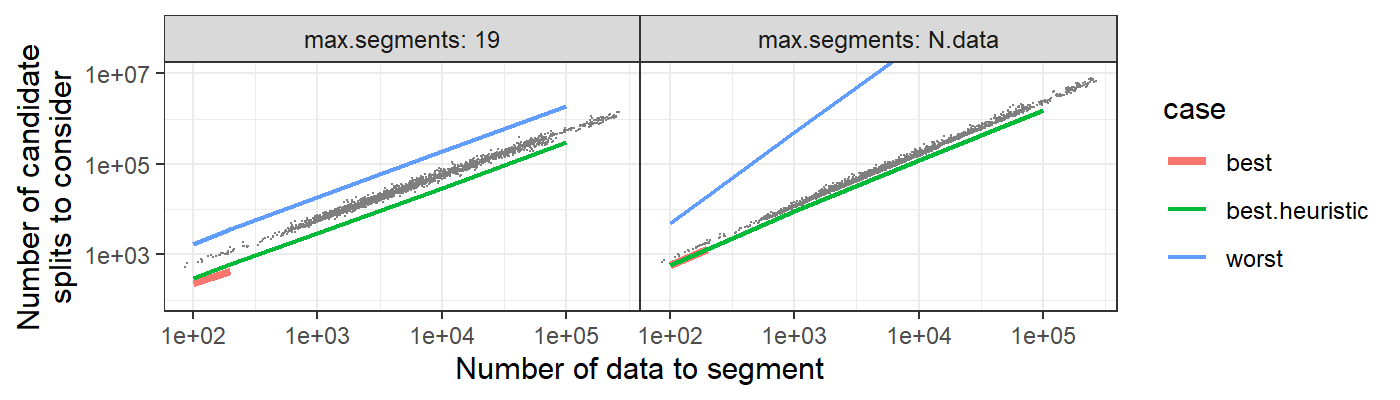
\includegraphics[width=\textwidth]{figure-mcgill-iterations.png}
   % \vspace{-0.7cm}
    \caption{\hl{Analysis} %MDPI: Please use scientific notations in the figure, e.g., “$8 \times 10^3$”, not “8E3”.
 of 2752 real genomic count data sets from McGill benchmark of data size $N$ from 87 to 263,169, using binary segmentation with the Poisson loss. 
% > range(iterations.dt$N.data)
% [1]     87 263169
    Number of candidate splits to consider in real data (grey dots) achieves the asymptotic best case, $O(N\log N)$.
    }
    \label{fig:mcgill-iterations}
\end{figure}

\subsubsection{\highlighting{Copy Number Benchmark}} 
We used data from R package neuroblastoma~\citep{neuroblastoma}, which is freely downloadable from the Comprehensive R Archive Network (CRAN) under the GPL-3 license.
This benchmark consists of 13,721 real genomic data sets of size $N$ from 11 to 5937.
We used the square loss since the data were real numbers.
We used R package binsegRcpp, and specified the max number of segments as either a constant (10), or equal to the number of data.
We used min segment length parameter $m=1$.
In these data we used Algorithm~\ref{algo:DP} to compute exact lower bounds for all data sizes $N$ from 11 to 100. 
We observed that the heuristic was always exact when max segments equals number of data, and it was exact for five sizes, $N\in\{11,12,13,18,19\}$, when max segments was set to 10.
As in the previous benchmark, we observed that the empirical number of splits that the algorithm considered closely matches the best case (Figure~\ref{fig:neuroblastoma-iterations}).
In fact we observed 45 real data sets for which the empirical number of splits considered was less than the heuristic/inexact lower bound.
Overall these data provide convincing evidence for fast performance in practical applications of binary segmentation.
In particular, in these real genomic data sets, binary segmentation is close to the best case asymptotic time complexity.

\begin{figure}[H]
    %\centering
    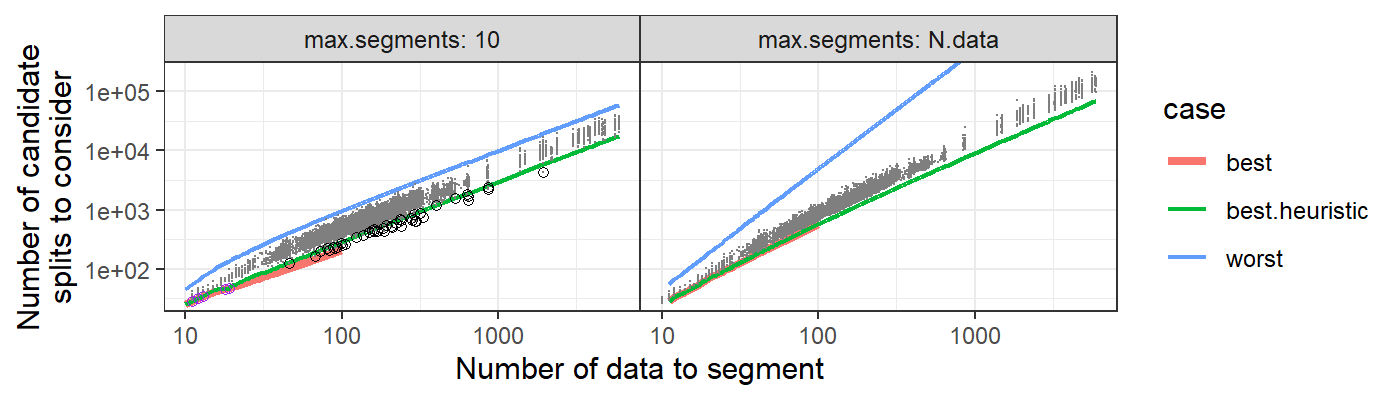
\includegraphics[width=\textwidth]{figure-neuroblastoma-iterations.png}
  %  \vspace{-0.7cm}
    \caption{\hl{Binary} %MDPI: Please use scientific notations in the figure, e.g., “$8 \times 10^3$”, not “8E3”.
 segmentation with the square loss was used on 13,721 real genomic data sets (grey dots) from the neuroblastoma benchmark with data sizes $N$ from 11 to 5937.
    Number of candidate splits to consider achieves the asymptotic best case, $O(N\log N)$, and in 45 instances (\hl{black} %MDPI: please confirm if grey dots need explanations?
 circles) requires fewer candidate splits than predicted by the best case heuristic.
    For max segments = 10, we used dynamic programming to compute the best case number of splits for all data sizes between 11 and 100 (orange line), and the heuristic (green line) was exact for only 5 data sizes $N\in\{11,12,13,18,19\}$ (purple circles).  }
    \label{fig:neuroblastoma-iterations}
\end{figure}

% > range(not.max$N.data)
% [1]   11 5937
% > nrow(not.max)
% [1] 13721
% > nrow(hilite)
% [1] 45
% > h.is.best
% Key: <max.segments, N.data, best>
%   max.segments N.data  best sum.splits_min sum.splits_max
%          <char>  <int> <int>          <int>          <int>
% 1:           10     11    29             30             42
% 2:           10     12    32             35             47
% 3:           10     13    35             40             49
% 4:           10     18    46             63             71
% 5:           10     19    48             62             97
% > nrow(bound.and.data[sum.splits==best]) #no best cases
% [1] 0

{\subsection{Analysis of Computation Time in Synthetic Data}
All timing results in this section depend on the particular computer hardware used; we used a laptop with a 2.40~GHz Intel(R) Core(TM)2 Duo CPU P8600.

\subsubsection{\textls[-25]{\highlighting{Similar Asymptotic Trends for Computation Time and Number of Candidate Splits}}}
To validate that candidate split count scales linearly with real computation time, we performed the following experiment.
We created synthetic best and worst case data sets for various data sizes $N$ from $10^1$ to $10^6$.
Best case data are linear, $x_i=i$; worst case data are alternating up and down, $x_i=1$ if $i$ is even and 0 if $i$ is odd.
On each data set, we ran binary segmentation, as implemented in the \texttt{wbs::sbs()} function in R, which computes the full path of splits using the square loss and min segment length $m=1$.
In this case, $K=N-1$, so we expected time and number of splits to be $O(N\log N)$ in the best case, and $O(N^2)$ in the worst case.
We used R package \texttt{atime} to compare timings and number of splits for various data sizes $N$, stopping after a time limit of 1 s~\citep{Amoakohene2026atime}.
Figure~\ref{fig:splits-time} shows that the empirical measurements (colored curves) closely match the asymptotic references (black curves).
These results clearly demonstrate that the number of splits considered by the algorithm scales linearly with real computation time.


\begin{figure}[H]
    %\centering
 \hspace{-7pt}   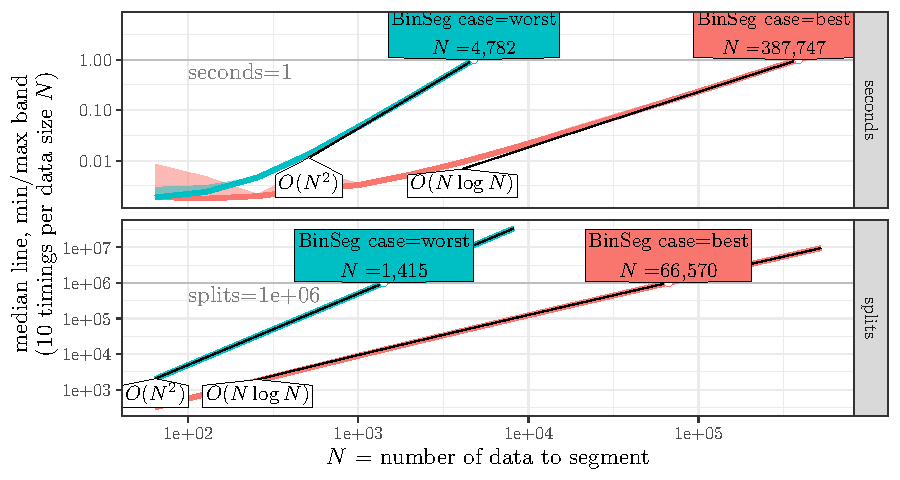
\includegraphics[width=\textwidth]{figure-splits-time.pdf}
    %\vspace{-0.7cm}
    \caption{\hl{Binary} %MDPI: 1. Commas are only used for numbers with five or more digits. Please remove them from the four-digit numbers in the figure, e.g., “1,200” should be “1200”.  2.  Please use scientific notations in the figure, e.g., “$8 \times 10^3$”, not “8E3”.
     segmentation with max changes ($K=N-1$ with min segment length $m=1$) was run for data sets of increasing sizes $N$, until going over the time limit of 1 s.
    Colored curves show timings (top) and number of candidate splits (bottom), for best and worst case synthetic data.
    Black lines show asymptotic references, which suggest that best case is $O(N\log N)$ time/splits, and worst case is $O(N^2)$.
    $N =$ values in colored boxes show throughput (data sizes computable given a limit of 1 s or $10^6$ splits).
    }
    \label{fig:splits-time}
\end{figure}


\subsubsection{\highlighting{Comparing Standard and Wild Binary Segmentation}}
To demonstrate the speed of binary segmentation relative to other changepoint methods, we performed the following experiment.
We created synthetic best case data ($x_i=i$) for various data sizes $N$ from $10^1$ to $10^6$.
On each data set, we ran standard binary segmentation (sbs) alongside wild binary segmentation (wbs), as implemented in the \texttt{sbs()} and \texttt{wbs()} functions in the R package \texttt{wbs}~\citep{fryzlewicz2014wild}.
Both functions compute a full path of splits using the square loss and min segment length $m=1$.
We ran \texttt{wbs()} using four diffirent settings for the number of intervals parameter $M$
 (two constants: $M = 10$ and the default $M = 5000$; two linearly increasing regimes: $M = N/2$ and $N/10$).
We expected the best case $O(N\log N)$ time complexity.
We used R package \texttt{atime} to compare timings for various data sizes $N$, stopping after a time limit of 1 s~\citep{Amoakohene2026atime}.
Figure~\ref{fig:wbs-sim-pred} shows that sbs has a convex timing curve that is consistent with the expected $O(N\log N)$ time complexity.
The wbs timing curves are non-convex, with an abrupt decrease in slope at 0.1 s, after which curves increase to their asymptotic regime.
It is clear that when M is constant (M~=~10 and the default M~=~5000), the wbs asymptotic slope is consistent with sbs, the expected best case $O(N\log N)$ time complexity.
Surprisingly, when M increases linearly (M~=~N/2 and N/10), the wbs asymptotic slope is larger, indicating $O(N^2)$ time, asymptotically slower than sbs.
The sbs algorithm is substantially faster than all wbs variants, for all N values.
Asymptotically, the closest wbs competitor is wbs with M~=~10, which is $\approx$10$\times$ slower than sbs.
These results clearly demonstrate that in best case data, standard binary segmentation is substantially faster than wild binary segmentation.

\begin{figure}[H]
    %\centering
    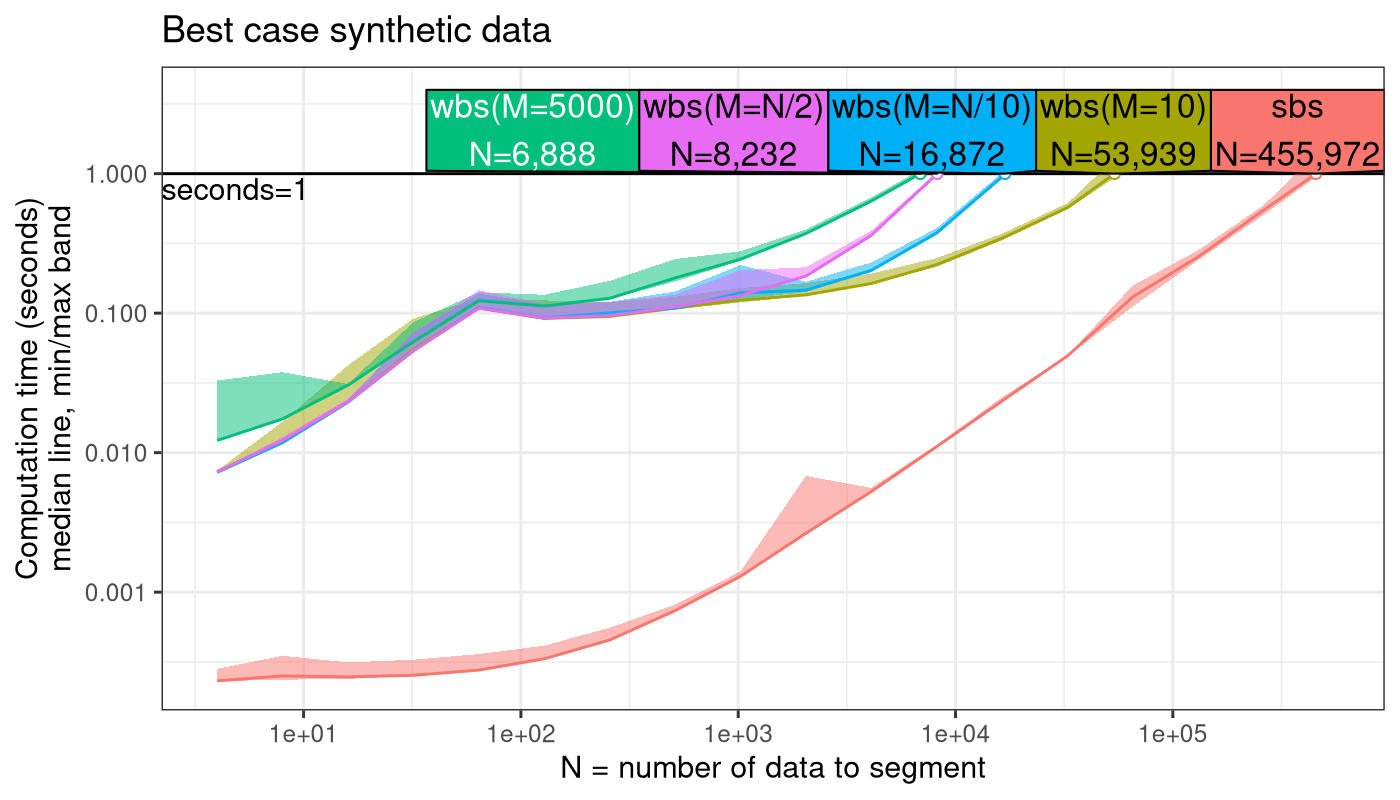
\includegraphics[width=0.98\textwidth]{figure-wbs-sim-pred.png}
    %\vspace{-0.7cm}
    \caption{\hl{Standard} %MDPI: 1. Commas are only used for numbers with five or more digits. Please remove them from the four-digit numbers in the figure, e.g., “1,200” should be “1200”.  2.  Please use scientific notations in the figure, e.g., “$8 \times 10^3$”, not “8E3”.
 binary segmentation (sbs) and wild binary segmentation (wbs), with max changes ($K=N-1$ with min segment length $m=1$), was run for data sets of increasing sizes $N$, until going over the time limit of 1 s.
    In these synthetic best case data, sbs is fastest, with asymptotic slope consistent with the expected $O(N\log N)$ time complexity for sbs, and for wbs with constant M parameter.
    For wbs with increasing M parameter (N/2 and N/10), the larger asymptotic slope is consistent with a larger asymptotic complexity class, $O(N^2)$.
    N = values in colored boxes show throughput (data sizes computable given a limit of 1 s).
    }
    \label{fig:wbs-sim-pred}
\end{figure}
}

\section{Discussion and Conclusions}
\label{sec:discussion}
This paper presented new methods for analyzing the time complexity of the classic binary segmentation algorithm for changepoint detection.
Our work analyzed the speed of the classic algorithm in terms of the number of candidate splits that must be considered in each iteration of the algorithm, and in terms of the number of previously computed splittable segments that must be stored. 
We proposed a new dynamic programming algorithm for computing a lower bound on the number of candidate splits that must be considered, thereby providing a method for finite sample analysis of the time complexity of the algorithm. 
We analyzed several real data sets in terms of the number of candidate splits that were computed, and compared those empirical observations to the upper and lower bounds.
We observed that in those real data sets, the empirical number of candidate splits is only a constant factor larger than the lower bound, indicating that the binary segmentation algorithm achieves the asymptotic best case in practical real data scenarios.
Our analysis provides convincing evidence that binary segmentation can be quickly computed for large real data sets, and large model sizes.
{Our work therefore suggests that the speed of binary segmentation is close to best case in several real data settings, $O(N \log K)$ time for $N$ data and $K$ segments.
Our empirical comparisons indicate slower speeds for wild binary segmentation~\citep{fryzlewicz2014wild}.
%\citep{fryzlewicz2014wild, kovacs2020seeded}.
}
One drawback/limitation of our work was the time complexity of our proposed dynamic programming algorithm, which was quadratic in both number of data and splits.
For future work, we plan to investigate faster algorithms for computing the best case lower bound, using ideas from the optimal binary search tree literature~\citep{NAGARAJ19971}.

% \paragraph{Author statement.} The authors declare that they have no conflict of interest. TDH contributed to the conception of ideas, proving theorems, implementing the algorithms, making figures, writing and revising the text.
% TODO


\vspace{6pt}


\funding{\hl{This research received no external funding. }}%Please add: ``'' or ``This research was funded by NAME OF FUNDER grant number XXX''. Check carefully that the details given are accurate and use the standard spelling of funding agency names at \url{https://search.crossref.org/funding}, any errors may affect your future funding.}


\dataavailability{
An R package with C/C++ code that implements our proposed algorithm is available \hl{at} %MDPI: Please provide the date you accessed the URL in the following format: “URL (accessed on Day Month Year)”. same below.
 \url{https://github.com/tdhock/binsegRcpp} (accessed 2 Sept 2026).
In addition, the \hl{GitHub} %MDPI: Please state which version of the software was used.
 \hl{repository} \url{https://github.com/tdhock/binseg-model-selection} contains code for reproducing the figures in this paper.
}%We encourage all authors of articles published in MDPI journals to share their research data. In this section, please provide details regarding where data supporting reported results can be found, including links to publicly archived datasets analyzed or generated during the study. Where no new data were created, or where data are unavailable due to privacy or ethical restrictions, a statement is still required. Suggested Data Availability Statements are available in the section ``MDPI Research Data Policies” at \url{https://www.mdpi.com/ethics}.} 


\conflictsofinterest{The authors declare no conflicts of interest.}%Declare conflicts of interest or state ``” Authors must identify and declare any personal circumstances or interests that may be perceived as inappropriately influencing the representation or interpretation of reported research results. Any role of the funders in the design of the study; in the collection, analyses or interpretation of data; in the writing of the manuscript; or in the decision to publish the results must be declared in this section. If there is no role, please state ``The funders had no role in the design of the study; in the collection, analyses, or interpretation of data; in the writing of the manuscript; or in the decision to publish the~results”.} 


\begin{adjustwidth}{-\extralength}{0cm}
%%\centering %% If there is a figure in wide page, please release command %\centering, for Table, ``\textwidth" should be ``\fulllength"
\reftitle{References}

\begin{thebibliography}{999}

\bibitem[Olshen et~al.(2004)Olshen, Venkatraman, Lucito, and
  Wigler]{olshen2004circular}
Olshen, A.B.; Venkatraman, E.; Lucito, R.; Wigler, M.
\newblock Circular binary segmentation for the analysis of array-based DNA copy
  number data.
\newblock {\em Biostatistics} {\bf 2004}, {\em 5},~557--572.

\bibitem[Killick et~al.(2010)Killick, Eckley, Ewans, and
  Jonathan]{killick2010detection}
Killick, R.; Eckley, I.A.; Ewans, K.; Jonathan, P.
\newblock Detection of changes in variance of oceanographic time-series using
  changepoint analysis.
\newblock {\em Ocean Eng.} {\bf 2010}, {\em 37},~1120--1126.

\bibitem[Fryzlewicz(2014)]{fryzlewicz2014wild}
Fryzlewicz, P.
\newblock Wild binary segmentation for multiple change-point detection.
\newblock {\em  Ann. Stat.} {\bf 2014}, {\em 42},~2243--2281.

\bibitem[Jewell et~al.(2019)Jewell, Hocking, Fearnhead, and Witten]{Jewell2019}
Jewell, S.W.; Hocking, T.D.; Fearnhead, P.; Witten, D.M.
\newblock {Fast nonconvex deconvolution of calcium imaging data}.
\newblock {\em Biostatistics} \hl{{\bf 2020}, \textit{21}, 709--726.} %MDPI: we change year 2019 into 2020, and add volume and pages, please confirm.


\bibitem[Auger and Lawrence(1989)]{segment-neighborhood}
Auger, I.; Lawrence, C.
\newblock Algorithms for the optimal identification of segment neighborhoods.
\newblock {\em Bull. Math. Biol.} {\bf 1989}, {\em 51},~39--54.

\bibitem[Jackson et~al.(2005)Jackson, Scargle, Barnes, Arabhi, Alt, Gioumousis,
  Gwin, Sangtrakulcharoen, Tan, and Tsai]{Jackson2005}
Jackson, B.; Scargle, J.; Barnes, D.; Arabhi, S.; Alt, A.; Gioumousis, P.;
  Gwin, E.; Sangtrakulcharoen, P.; Tan, L.; Tsai, T.
\newblock An algorithm for optimal partitioning of data on an interval.
\newblock {\em IEEE Signal Process Lett.} {\bf 2005}, {\em 12},~105--108.

\bibitem[Maidstone et~al.(2016)Maidstone, Hocking, Rigaill, and
  Fearnhead]{Maidstone2016}
Maidstone, R.; Hocking, T.; Rigaill, G.; Fearnhead, P.
\newblock On optimal multiple changepoint algorithms for large data.
\newblock {\em Stat. Comput.}  \hl{\textbf{2017}, \textit{27}, 519--533.} %MDPI: we change {\bf 2016}, pp. 1--15 into it, please confirm.


\bibitem[Scott and Knott(1974)]{binary-segmentation}
Scott, A.; Knott, M.
\newblock A cluster analysis method for grouping means in the analysis of
  variance.
\newblock {\em Biometrics} {\bf 1974}, {\em 30},~507--512.

\bibitem[Baranowski et~al.(2019)Baranowski, Chen, and
  Fryzlewicz]{baranowski2019narrowest}
Baranowski, R.; Chen, Y.; Fryzlewicz, P.
\newblock Narrowest-over-threshold detection of multiple change points and
  change-point-like features.
\newblock {\em J. R. Stat. Soc. Ser. B (Stat. Methodol.)} {\bf 2019}, {\em 81},~649--672.

\bibitem[Kov{\'a}cs et~al.(2020)Kov{\'a}cs, Li, B{\"u}hlmann, and
  Munk]{kovacs2020seeded}
Kov{\'a}cs, S.; Li, H.; B{\"u}hlmann, P.; Munk, A.
\newblock Seeded binary segmentation: A general methodology for fast and
  optimal change point detection.
\newblock {\em arXiv} {\bf 2020}, arXiv:2002.06633.

\bibitem[Venkatraman(1992)]{venkatraman1992consistency}
Venkatraman, E.
\newblock Consistency Results in Multiple Change-Point Situations.
\newblock {Unpublished Ph.D. Thesis, Department of Statistics, Stanford  University, \hl{Stanford, CA, USA,} %MDPI: Newly added  information. Please confirm. The same to following highlight.
 1992}.

\bibitem[Levin and Kline(1985)]{levin1985cusum}
Levin, B.; Kline, J.
\newblock The cusum test of homogeneity with an application in spontaneous
  abortion epidemiology.
\newblock {\em Stat. Med.} {\bf 1985}, {\em 4},~469--488.

\bibitem[Breiman et~al.(1984)Breiman, Friedman, Olshen, and
  Stone]{breiman1984classification}
Breiman, L.; Friedman, J.H.; Olshen, R.A.; Stone, C.J.
\newblock {\em Classification and Regression Trees}; Routledge: \hl{London, UK,} 1984.

\bibitem[Drouin et~al.(2017)Drouin, Hocking, and Laviolette]{Drouin2017}
Drouin, A.; Hocking, T.; Laviolette, F.
\newblock Maximum Margin Interval Trees. In {\em Advances in Neural Information
  Processing Systems 30}; Guyon, I., Luxburg, U.V., Bengio, S., Wallach, H.,
  Fergus, R., Vishwanathan, S., Garnett, R., Eds.; Curran Associates, Inc.: \hl{New~York, NY, USA,}  2017; pp. 4947--4956.

\bibitem[Yao(1988)]{Yao88}
Yao, Y.C.
\newblock {Estimating the number of change-points via Schwarz' criterion}.
\newblock {\em Stat. Probab. Lett.} {\bf 1988}, {\em
  6},~181--189.

\bibitem[Zhang and Siegmund(2007)]{mBIC}
Zhang, N.R.; Siegmund, D.O.
\newblock {A Modified Bayes Information Criterion with Applications to the
  Analysis of Comparative Genomic Hybridization Data}.
\newblock {\em Biometrics} {\bf 2007}, {\em 63},~22--32.

\bibitem[Rigaill et~al.(2013)Rigaill, Hocking, Vert, and Bach]{Hocking2013icml}
Rigaill, G.; Hocking, T.; Vert, J.P.; Bach, F.
\newblock Learning sparse penalties for change-point detection using max margin
  interval regression.
\newblock In Proceedings of the 30th \hl{International Conference on Machine Learning,} %MDPI: We add full names, please confirm.
 \hl{Atlanta, GA,  USA, 16--21 June} 2013; \mbox{pp. 172--180.}

\bibitem[Truong et~al.(2017)Truong, Gudre, and Vayatis]{truong2017penalty}
Truong, C.; Gudre, L.; Vayatis, N.
\newblock Penalty learning for changepoint detection.
\newblock In \textit{Proceedings of the 2017 25th European Signal Processing Conference
  (EUSIPCO)}; IEEE: \hl{New York, NY, USA,} 2017; pp. 1569--1573.

\bibitem[Nagaraj(1997)]{NAGARAJ19971}
Nagaraj, S.
\newblock Optimal binary search trees.
\newblock {\em Theor. Comput. Sci.} {\bf 1997}, {\em 188},~1--44.
\newblock
  {\url{https://doi.org/https://doi.org/10.1016/S0304-3975(96)00320-9}}.

\bibitem[Knuth(1971)]{Knuth1971}
Knuth, D.E.
\newblock Optimum binary search trees.
\newblock {\em Acta Inform.} {\bf 1971}, {\em 1},~14--25.
\newblock {\url{https://doi.org/10.1007/BF00264289}}.

\bibitem[Mehlhorn(1975)]{mehlhorn1975nearly}
Mehlhorn, K.
\newblock Nearly optimal binary search trees.
\newblock {\em Acta Inform.} {\bf 1975}, {\em 5},~287--295.

\bibitem[Hocking et~al.(2016)Hocking, Goerner-Potvin, Morin, Shao, Pastinen,
  and Bourque]{Hocking2017bioinfo}
Hocking, T.D.; Goerner-Potvin, P.; Morin, A.; Shao, X.; Pastinen, T.; Bourque,
  G.
\newblock {Optimizing ChIP-seq peak detectors using visual labels and
  supervised machine learning}.
\newblock {\em Bioinformatics} {\bf 2016}, {\em 33},~491--499.

\bibitem[Hocking(2013)]{neuroblastoma}
Hocking, T.D.
\newblock {\em Neuroblastoma: Neuroblastoma Copy Number Profiles}; R Package Version 1.0;  \hl{2013.} %MDPI: We are sorry but we could not find the required information about this entry. Please add the name of the publisher and their location.

 

\bibitem[Amoakohene et~al.(2026)Amoakohene, Chetia, Steinmacher, and
  Hocking]{Amoakohene2026atime}
Amoakohene, D.; Chetia, A.; Steinmacher, I.; Hocking, T.
\newblock Asymptotic benchmarking using the atime package.
\newblock {\em R J.} {\bf 2026}, {\em 18},~170--188.

\end{thebibliography}
\PublishersNote{}
\end{adjustwidth}

\end{document}

